%!TEX program = xelatex

\documentclass[compress]{beamer}
%--------------------------------------------------------------------------
% Common packages
%--------------------------------------------------------------------------

\definecolor{links}{HTML}{663000}
\hypersetup{colorlinks,linkcolor=,urlcolor=links}

\usepackage[english]{babel}
\usepackage{pgfpages} % required for notes on second screen
\usepackage{graphicx}

\usepackage{pdfpcnotes}

\usepackage{multicol}

\usepackage{tabularx,ragged2e}
\usepackage{booktabs}

\setlength{\emergencystretch}{3em}  % prevent overfull lines
\providecommand{\tightlist}{%
  \setlength{\itemsep}{0pt}\setlength{\parskip}{0pt}}


\usetheme{hri}

% Display the navigation bullet even without subsections
\usepackage{remreset}% tiny package containing just the \@removefromreset command
\makeatletter
\@removefromreset{subsection}{section}
\makeatother
\setcounter{subsection}{1}

\makeatletter
\let\beamer@writeslidentry@miniframeson=\beamer@writeslidentry
\def\beamer@writeslidentry@miniframesoff{%
  \expandafter\beamer@ifempty\expandafter{\beamer@framestartpage}{}% does not happen normally
  {%else
    % removed \addtocontents commands
    \clearpage\beamer@notesactions%
  }
}
\newcommand*{\miniframeson}{\let\beamer@writeslidentry=\beamer@writeslidentry@miniframeson}
\newcommand*{\miniframesoff}{\let\beamer@writeslidentry=\beamer@writeslidentry@miniframesoff}
\makeatother



\newcommand{\source}[2]{{\tiny\it Source: \href{#1}{#2}}}

\usepackage{tikz}
\usetikzlibrary{mindmap,backgrounds,positioning,calc,patterns}
\usepackage{pgfplots}
\pgfplotsset{compat=newest}
\usepackage{circuitikz}

\usepackage[normalem]{ulem}

\graphicspath{{figs/}}

\title{ROCO222 \newline Intro to Sensors and Actuators}
\subtitle{Stepper motors}

\date{}
\author{Séverin Lemaignan}
\institute{Centre for Neural Systems and Robotics\\{\bf Plymouth University}}

\begin{document}

\licenseframe{github.com/severin-lemaignan/module-introduction-sensors-actuators}

\maketitle

\miniframesoff
\begin{frame}{What have we done so far?}

\begin{itemize}
    \item \textbf{Week 1} -- \sout{Arduino + Encoders}
    \item \textbf{Week 2} -- \sout{Electromagnetism and DC motors 1}
    \item \textbf{Week 4} -- \sout{Electromagnetism and DC motors 2}
    \item \textbf{Week 5} -- \sout{Magnets, brushless motor, motor control}
    \item \textbf{Week 6} -- Stepper motors
    \item \textbf{Week 7} -- \emph{no lecture}
    \item \textbf{Week 8} -- Non-electrical actuators (Martin Stoelen)
    \item \textbf{Week 9} -- ROS middleware, joint state, kinematics 101, visualisation
    \item \textbf{Week 10} -- Software engineering for robotics
    \item \textbf{Week 11} -- Induction motors
    \item \textbf{Week 12} -- Sensors
    \item \textbf{Week 13} -- Exam preparation
\end{itemize}

\end{frame}

\begin{frame}{Labs}

\begin{itemize}
    \item \textbf{Week 1} -- \sout{Git, Linux, command-line}
    \item \textbf{Week 2} -- \sout{DC motor design}
    \item \textbf{Week 4} -- \sout{Incremental encoder}
    \item \textbf{Week 5} -- \sout{Arduino motor control}
    \item \textbf{Week 6} -- Arduino and Stepper motors
    \item \textbf{Week 7} -- \textbf{Lab on Monday for everyone} Servo project intro
    \item \textbf{Week 8} -- Design for 3D printing (Jake)
    \item \textbf{Week 9} -- Servo project cont'd
    \item \textbf{Week 10} -- Servo project cont'd
    \item \textbf{Week 11} -- Servo project cont'd
    \item \textbf{Week 12} -- Servo project final
\end{itemize}

\end{frame}


\miniframeson



\section{Stepper motors}

\begin{frame}{Stepper motor basic principle}
    \begin{columns}
        \begin{column}{0.4\linewidth}
            \begin{center}
                \includegraphics[width=1.2\linewidth]{bipolar}
            \end{center}
        \end{column}
        \begin{column}{0.6\linewidth}
            \begin{itemize}
                \item A stepper motor is a synchronous electric motor.
                \item The rotor's equilibrium position occurs when aligned with the
                    stator's magnetic field
                \item By sequencing the current in the coils, one generates a rotating
                    magnetic field, which in turn generates a rotation of the
                    rotor, one step at time.
            \end{itemize}
        \end{column}
    \end{columns}

\end{frame}

{\fullbackground[scale=0.9,page=3]{ian-stepper-motors.pdf}
    \begin{frame}{Several basic types of stepping motors}
    \end{frame}
}

{\fullbackground[scale=0.9,page=4]{ian-stepper-motors.pdf}
    \begin{frame}{Variable reluctance motor}
    \end{frame}
}

{\fullbackground[scale=0.9,page=5]{ian-stepper-motors.pdf}
    \begin{frame}{Variable reluctance stepper motor operation}
    \end{frame}
}

{\fullbackground[scale=0.9,page=6]{ian-stepper-motors.pdf}
    \begin{frame}{Variable reluctance stepper motor: sequencing}
    \end{frame}
}

{\fullbackground[scale=0.9,page=7]{ian-stepper-motors.pdf}
    \begin{frame}{Variable reluctance motor coils}
    \end{frame}
}

{\fullbackground[scale=0.9,page=9]{ian-stepper-motors.pdf}
    \begin{frame}{Permanent magnet stepper motor}
    \end{frame}
}

{\fullbackground[scale=0.9,page=10]{ian-stepper-motors.pdf}
    \begin{frame}{Permanent magnet stepper motor features}
    \end{frame}
}

\begin{frame}{Hybrid stepper motors}

    \begin{columns}
        \begin{column}{0.6\linewidth}
            \begin{itemize}
                \item combine a permanent magnet and a
                    rotor with metal teeth to provide features of the variable
                    reluctance and permanent magnet motors 

                \item the rotor teeth provide a smaller magnetic circuit
                    resistance in some rotor positions, which improves static
                    and dynamic torque

                \item more expensive than other steppers, but they use smaller
                    steps, have greater torque, and have greater maximum speeds

                \item most common type of stepper
            \end{itemize}
        \end{column}
        \begin{column}{0.4\linewidth}

            \begin{center}
                \includegraphics[width=0.9\linewidth]{hybrid}
                \hspace{1em}

                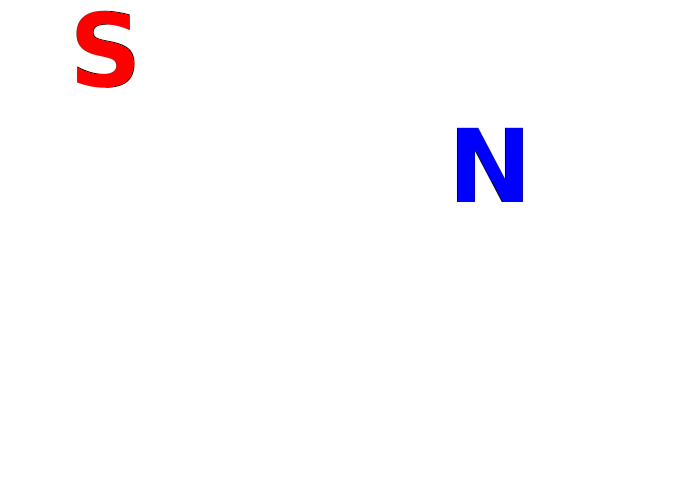
\includegraphics[width=0.9\linewidth]{magnetized-shaft}
            \end{center}
        \end{column}
    \end{columns}

\end{frame}

\begin{frame}{Hybrid stepping motor operation}
    \begin{center}
        \begin{columns}
            \begin{column}{0.5\linewidth}
        \includegraphics[width=\linewidth]{hybrid}

        \source{https://www.phidgets.com/docs/Stepper_Motor_and_Controller_Primer}{Phidgets.com (check the link for details)}
                
            \end{column}
            \begin{column}{0.5\linewidth}
        \includegraphics[width=\linewidth]{hybrid-operation}

        \source{http://www.nmbtc.com/step-motors/engineering/construction-and-operating-theory/}{MinebeaMitsumi}
             \end{column}
        \end{columns}

    \end{center}

    \pnote{
        The image to the right is a cross-sectional view of the inside of a
        hybrid bipolar stepper motor. As you can see, it has eight poles with
        six teeth each. This motor contains two coils- one wrapping the
        odd-numbered poles, and the other wrapping the even-numbered poles. The
        steel end-cap in the center of the image covers a cylindrical permanent
        magnet which surrounds the shaft.

        If positive current is sent to the odd-numbered coil, poles 1 and 5 are
        magnetized as south, and poles 3 and 7 are magnetized as north. Assuming
        the permanent magnet in the center of the motor has its north pole
        facing toward us, this will result in the rotor turning so that the
        teeth line up with stator poles 1 and 5, as they are in the image. At
        the same time, poles 3 and 7 will become aligned on the opposite end of
        the motor, where the gear on the rotor is permanently offset by the
        width of one tooth and the permanent magnet has magnetized the rotor as
        south. The rotation of the motor is continued by sending negative
        current through the even-numbered phase, then negative current through
        the odd-numbered phase, then positive current through the even-numbered
        phase, and so on. The stepper controller can reverse the direction of
        rotation simply by reversing this sequence.

        When a stepper motor becomes engaged in software, and current is applied
        to the coils, it may abruptly "snap" to the position that the rotor is
        being held at. 
    }
\end{frame}

\imageframe{parts-hybrid}


\begin{frame}{Bipolar motor windings}

    \begin{columns}
        \begin{column}{0.5\linewidth}

            \begin{center}
                \includegraphics[width=\linewidth]{bipolar}
            \end{center}
        \end{column}
        \begin{column}{0.5\linewidth}

            \begin{itemize}
                \item In a bipolar winding the current flow on the coils is reversed, which reverses electromagnetic polarity
                \item All the windings can be used to drive the motor
                \item Four wires 
                \item No common center connection. 
                \item Two independent sets of coils
                \item Need H-bridge to reverse direction of current in coils
            \end{itemize}
        \end{column}
    \end{columns}

\end{frame}

\begin{frame}{Unipolar motor windings}


    \begin{center}
        \includegraphics[width=0.6\linewidth]{unipolar}
    \end{center}

    \only<1>{
    Unipolar stepping motor are made of two windings.

        \begin{itemize}
            \item Each windings has a center tap either brought outside motor
                separately or connected together and brought outside as one wire

            \item Therefore unipolar motors have 5 or 6 wires
        \end{itemize}
    }
    \only<2>{
        \begin{itemize}
            \item Center taps normally tied to GND, ends of the coils alternately V+ 
            \item Unipolar drivers always energize the coils in the same direction.
            \item Current flow is never reversed, hence the name unipolar
            \item Less available torque because only half of the coils energized at a time
        \end{itemize}
    }
\end{frame}

{\fullbackground[scale=0.9,page=17]{ian-stepper-motors.pdf}
    \begin{frame}{Bipolar delivers more torque than unipolar}
    \end{frame}
}


{\fullbackground[scale=0.9,page=19]{ian-stepper-motors.pdf}
    \begin{frame}{Bifilar stepper motor}
    \end{frame}
}

\section[Arduino]{Controlling a stepper motor with an Arduino}

\begin{frame}{Unipolar versus bipolar circuitry}

    \begin{center}
        \includegraphics[width=0.6\linewidth]{wiring}
    \end{center}

    \small
    \begin{columns}
        \begin{column}{0.6\linewidth}
            \begin{itemize}
                \item Only need simple switching units to operate
                \item Don’t need H-bridge
                \item Unipolar drivers can be implemented with simple transistor circuitry
            \end{itemize}
        \end{column}
        \begin{column}{0.5\linewidth}
            \begin{itemize}
                \item Bipolar drivers need H-bridge circuitry to reverse the current flow though the coil
                \item \emph{Not really a problem these days!}
            \end{itemize}
        \end{column}
    \end{columns}
\end{frame}

\begin{frame}{Colour coding}

    \begin{center}
        \includegraphics[width=0.75\linewidth]{color-codes}

        \source{https://www.linengineering.com/}{Lin engineering}
    \end{center}
\end{frame}


\begin{frame}{Wiring to the Arduino motor shield}

    \begin{center}
        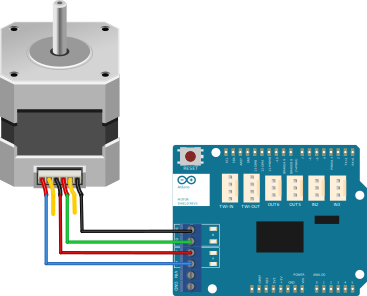
\includegraphics[width=0.8\linewidth]{unipolar-wiring}
    \end{center}
\end{frame}

\begin{frame}[fragile]{Full-step control program}
    \begin{overprint}
    \onslide<1>
        \begin{minted}[frame=none,
               linenos=false,
               fontsize=\small,
               xleftmargin=0.5em]{cpp}

#define DIR_A 12
#define PWM_A 3
#define DIR_B 13
#define PWM_B 11

const int delayMs = 100;

void setup() {
  pinMode(DIR_A, OUTPUT);
  pinMode(DIR_B, OUTPUT);

  pinMode(9, OUTPUT); digitalWrite(8, LOW); //No braking ch. A
  pinMode(8, OUTPUT); digitalWrite(8, LOW); //No braking ch. B
}

\end{minted}
\onslide<2>
\begin{minted}[frame=none,
               linenos=false,
               fontsize=\scriptsize,
               xleftmargin=0.5em]{cpp}
void loop(){

  digitalWrite(DIR_A, HIGH); // Ch. A forward
  digitalWrite(DIR_B, HIGH); // Ch. B forward
  analogWrite(PWM_A, 255); // Ch. A on
  analogWrite(PWM_B, 0); // Ch. B off
  delay(delayMs);
  
  analogWrite(PWM_A, 0); // Ch. A off
  analogWrite(PWM_B, 255); // Ch. B on
  delay(delayMs);
  
  digitalWrite(DIR_A, LOW); // Ch. A backwards
  digitalWrite(DIR_B, LOW); // Ch. B backwards
  analogWrite(PWM_A, 255); // Ch. A on
  analogWrite(PWM_B, 0); // Ch. B off
  delay(delayMs);
  
  analogWrite(PWM_A, 0); // Ch. A off
  analogWrite(PWM_B, 255); // Ch. B on
  delay(delayMs);
}
\end{minted}
        \end{overprint}
\end{frame}

\videoframe[0.56]{figs/stepper.mov}

\section[Modes]{Stepper motor modes}

{\fullbackground[scale=0.9,page=21]{ian-stepper-motors.pdf}
    \begin{frame}{Stepping motor control modes}
    \end{frame}
}
{\fullbackground[scale=0.9,page=22]{ian-stepper-motors.pdf}
    \begin{frame}{Full step operation}
    \end{frame}
}

{\fullbackground[scale=0.9,page=24]{ian-stepper-motors.pdf}
    \begin{frame}{2 Phases full step operation}
    \end{frame}
}

{\fullbackground[scale=0.9,page=23]{ian-stepper-motors.pdf}
    \begin{frame}{Half step operation}
    \end{frame}
}

{\fullbackground[scale=0.9,page=25]{ian-stepper-motors.pdf}
    \begin{frame}{Single step response and resonances}
    \end{frame}
}

{\fullbackground[scale=0.9,page=26]{ian-stepper-motors.pdf}
    \begin{frame}{Microstepping}
    \end{frame}
}

{\fullbackground[scale=0.9,page=27]{ian-stepper-motors.pdf}
    \begin{frame}{Sine-cosine microstepping}
    \end{frame}
}

{\fullbackground[scale=0.9,page=28]{ian-stepper-motors.pdf}
    \begin{frame}{Arduino microstepping example code}
    \end{frame}
}

{\fullbackground[scale=0.9,page=29]{ian-stepper-motors.pdf}
    \begin{frame}{Arduino microstepping example code}
    \end{frame}
}

\section[Characterisation]{Characterisation of stepper motors}

{\fullbackground[scale=0.9,page=30]{ian-stepper-motors.pdf}
    \begin{frame}{Stepper motor step parameters}
    \end{frame}
}

{\fullbackground[scale=0.9,page=31]{ian-stepper-motors.pdf}
    \begin{frame}{Example: step parameters}
    \end{frame}
}
{\fullbackground[scale=0.9,page=32]{ian-stepper-motors.pdf}
    \begin{frame}{Current flow in stepper motors}
    \end{frame}
}

{\fullbackground[scale=0.9,page=33]{ian-stepper-motors.pdf}
    \begin{frame}{Current flow in stepper motors}
    \end{frame}
}

{\fullbackground[scale=0.9,page=34]{ian-stepper-motors.pdf}
    \begin{frame}{Current flow in stepper motors}
    \end{frame}
}

{\fullbackground[scale=0.9,page=35]{ian-stepper-motors.pdf}
    \begin{frame}{Chopper control of current}
    \end{frame}
}

{\fullbackground[scale=0.9,page=36]{ian-stepper-motors.pdf}
    \begin{frame}{Rough calculation of max pulse rate}
    \end{frame}
}

{\fullbackground[scale=0.9,page=37]{ian-stepper-motors.pdf}
    \begin{frame}{Rough calculation of max pulse rate}
    \end{frame}
}

{\fullbackground[scale=0.9,page=38]{ian-stepper-motors.pdf}
    \begin{frame}{Stepper motor torque-speed characteristic}
    \end{frame}
}

{\fullbackground[scale=0.9,page=39]{ian-stepper-motors.pdf}
    \begin{frame}{Stepper motor torque-speed characteristic}
    \end{frame}
}

{\fullbackground[scale=0.9,page=40]{ian-stepper-motors.pdf}
    \begin{frame}{Stepper motor torque-speed characteristic}
    \end{frame}
}

%%%%%%%%%%%%%%%%%%%%%%%%%%%%%%%%%%%%%%%%%%%%%%%%%%%%%%%%%%%%%%%%%%%%%%%%
%%%%%%%%%%%%%%%%%%%%%%%%%%%%%%%%%%%%%%%%%%%%%%%%%%%%%%%%%%%%%%%%%%%%%%%%
%%%%%%%%%%%%%%%%%%%%%%%%%%%%%%%%%%%%%%%%%%%%%%%%%%%%%%%%%%%%%%%%%%%%%%%%
\section[Drivers]{Stepper motor drivers}

{\fullbackground[scale=0.9,page=42]{ian-stepper-motors.pdf}
    \begin{frame}{L298N DC stepper motor controller}
    \end{frame}
}

{\fullbackground[scale=0.9,page=43]{ian-stepper-motors.pdf}
    \begin{frame}{L298N DC stepper motor controller}
    \end{frame}
}

{\fullbackground[scale=0.9,page=44]{ian-stepper-motors.pdf}
    \begin{frame}{L298N DC stepper motor controller}
    \end{frame}
}

{\fullbackground[scale=0.9,page=45]{ian-stepper-motors.pdf}
    \begin{frame}{L298N DC stepper motor controller}
    \end{frame}
}

\begin{frame}{On the Arduino motor shield}
    \begin{center}
        \includegraphics[width=0.8\linewidth]{motorshield}
    \end{center}
\end{frame}

{\fullbackground[scale=0.9,page=47]{ian-stepper-motors.pdf}
    \begin{frame}{DRV8825 stepper motor controller}
    \end{frame}
}

{\fullbackground[scale=0.9,page=48]{ian-stepper-motors.pdf}
    \begin{frame}{DRV8825 stepper motor controller}
    \end{frame}
}

\section[Limits]{Strenghts and Weaknesses}

{\fullbackground[scale=0.9,page=50]{ian-stepper-motors.pdf}
    \begin{frame}{Advantages and disadvantages of steppers}
    \end{frame}
}

{\fullbackground[scale=0.9,page=51]{ian-stepper-motors.pdf}
    \begin{frame}{Advantages and disadvantages of steppers}
    \end{frame}
}
{\fullbackground[scale=0.9,page=52]{ian-stepper-motors.pdf}
    \begin{frame}{Stepper motor design issues}
    \end{frame}
}

{\fullbackground[scale=0.9,page=53]{ian-stepper-motors.pdf}
    \begin{frame}{Typical stepper torque characteristics}
    \end{frame}
}

\section{Applications}

{\fullbackground[scale=0.9,page=56]{ian-stepper-motors.pdf}
    \begin{frame}{Wide range of standard NEMA frames}
    \end{frame}
}

\begin{frame}{Variable number of stacks}

    \begin{center}
        \includegraphics[width=0.8\linewidth]{stepper-stacks-size}
    \end{center}
\end{frame}

{\fullbackground[scale=0.9,page=54]{ian-stepper-motors.pdf}
    \begin{frame}{CNC mill using steppers}
    \end{frame}
}

\videoframe[0.56]{../part4/figs/3d-printer.mp4}

{\fullbackground[scale=0.9,page=55]{ian-stepper-motors.pdf}
    \begin{frame}{Servo motor versus stepper motor}
    \end{frame}
}

{\fullbackground[scale=0.9,page=57]{ian-stepper-motors.pdf}
    \begin{frame}{Geared stepper motor}
    \end{frame}
}

\imageframe[color=black]{datasheet}

\begin{frame}{}
    \begin{center}
        \Large
        That's all, folks!\\[2em]
        \normalsize
        Questions:\\
        Portland Square B316 or \url{severin.lemaignan@plymouth.ac.uk} \\[1em]

        Slides:\\
        \href{https://github.com/severin-lemaignan/module-introduction-sensors-actuators}{\small
        github.com/severin-lemaignan/module-introduction-sensors-actuators}


    \end{center}
\end{frame}



\end{document}
